% Implementation (4000 words)
% * Refer to design strategies that looked ahead to the testing stage
% * Draw attention to what is not my own work (ie rebar, webmachine etc)
% * Major milestones might be highlighted with advantage
% *! Show evidence of skill, clear thinking and common sense

% ************
% Should have: 
% 	intro
% 	content
% 	summary
% ************

% Word budget 4000 words. Try to keep it less
\section{Implementation}

Intro

% Content
%   What is to be stored
%     How do we solve search across key's?
%     How much space does this take up?
%       Average name length?
%       Amount of data per user?

\subsection{General discussion}
Before I start discussing how I implemented my project, I want to discuss what data I am interested in storing in my search network, and how I built a search index on top of a distributed hash table. 

\mbox{}

My search network stores records with information about users, much like a normal address book does. I made the following fields mandatory: the person's name, a url to her online social network profile page, and a url to a profile image that can be displayed alongside the search result.

For the purpose of this project I did not want to lock down exactly what data should be stored, but before my system is used in a wider context it would be wise to look into using some well known public standard. At this stage it is outside the scope of my project.

As I briefly discussed in the preparation chapter, a key-value store does not immediately lend itself to search. If you don't know the key under which a data item is stored, you would have to do a linear search across the keyspace in order to find what you are looking for. The solution is to use the persons name as the key. Human names in their natural form do not easily map uniformly onto any keyspace. They are of different length and also cluster around more common names. I therefore used a hashing function to hash names into keys. This immediately presents us with another problem. If you don't know the exact spelling of the name that was used to generate the key you still can't get around a linear search through the datastore. You can partly solve this problem by normalising names before hashing them into keys, but the utility of a search engine that requires you to already know a complete and correct match of what you are looking for is arguably rather low. Users today increasignly expect search engines to deliver predictive searches where results show before you finish typing your search query. This scheme does neither accommodate this, nor misspelled names, or for that matter cases where you have forgotten your friends middle name.

I solved the problem in the following way: Instead of storing just profile records I store both \emph{profile records} and \emph{link records}. The profile records contain all the information about the user and are stored under a key generated by hashing the whole record. The link records on the other hand are lightweight pointers to the full records. They contain the full name and the key of the profile record, and are stored under a key generated by a subset of the name. Each profile record has multiple link records pointing at it. I will come back to how I am generating these link records shortly.

Using link records solves several problems. By storing links keyed by fragments of a users name, the search engine can start looking up information before the user has completed typing the search phrase. This enables predictive search. Since the link records also contain the full name of the user you can detect and work around misspelled names, or even searches that don't include all the users names.

% How link records are generated
\begin{figure}[htb]
\begin{center}
	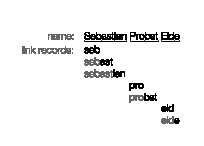
\includegraphics[width=0.6\linewidth]{illustrations/LinkRecords.eps}
\caption{Here it is shown how a name maps into name fragments used for storing link records pointing to a profile record.}
\label{figLinkRecord}
\end{center}
\end{figure}

In the current implementation I create link records for each three additional characters contained in a users name. This is illustrated in figure \ref{figLinkRecord}. The process is done separately for each name. First the first three characters of a name is taken. Then for the next key the subsequent three characters are added. This process is repeated until you reach the end of a name. When you reach the end of a name that is not a multiple of 3, an additional link record is created for the full length of the name. In the example you see this illustrated in how Eide results in the link records \emph{eid} and \emph{eide}.

Using link records does generate extra overhead when searching. A search will now no longer require a single lookup in the search index, but several. As the user types the search server will have to look up link records and resolve them to their profile records. If you searched for my full name, a total of 9 requests would have to be made. 8 for each of the link entries, and an additional one for looking up the full record with all the information about the user. 

In reality it isn't quite as bad as it sounds. The desired result is likely to show up before the user has finished typing, in which case there won't be additional lookups for the remaining link items. 

The link items also let the search server rank results by relevance. Let me illustrate this with another example. Say the system contains two profile records: one for Probst and one for Probstonius. If you search for Probst you get two link records, one for pro and one for probst. Both will return pointers to the profile records of both Probst and Probstonius. Since Probst is a complete match for the search term \emph{probst} while Probstonius is only a partial match, the result for Probst can be given a higher relevance score. The current implementation does this.

<<<DISCUSS COST OF THIS>>>

%   Parts not my own
%     Rebar build system
%     Webmachine http arbitrator
%     OTP
%       gen_server
%       supervisors

\subsection{Third party code used}
In this section I want to briefly discuss what third party projects I was using in my project.

Most prominent is my dependence on OTP, the Open Telecom Platform, part of the Erlang standard distribution. It is a set of libraries that provide basic functionality needed to write amongst others general servers, and provide functionality for supervising processes within your application and restarting them when they fail. Most Erlang applications rely on OTP.

I also used Webmachine, an open source framework for creating HTTP interfaces in Erlang, and rebar, a build system. Both are developed by Basho.

For testing I used EUnit, part of the standard Erlang distribution, for regular functional unit tests and Erlymock for testing functions with side effects where I wanted to control the functions interactions with the environment.


%   Methology
%     Test driven development
%     Integration testing for gen_server
%   Made it modular.
%   Swappable DHT

\subsection{Process}
At this time it is well understood how Distributed Hash Tables work. The bulk of research in Distributed Hash Tables was done around year 2000. The research papers presenting Chord and Pastry also supply high level code that I referenced when implementing the algorithms. This provided an excellent foundation for doing test-driven development. All the core components of my system were unit tested, and in the tradition of test-driven development I wrote the minimal code needed to satisfy my tests. This encourages writing modular systems with self-contained and side effect free functions.
I wrote additional integration tests where I felt it served a purpose.

Modularity was also a key design factor for other reasons. I wanted as many as possible of my modules to be ignorant of which Distributed Hash Table was being used. This encouraged me to keep the interface between the Distributed Hash Tables and the surrounding code strict and minimal. In effect the only methods the Distributed Hash Table's need to export are ways to get and set values by key.


%   Components of the system
%     Client side
%       Backend
%         Controller
%         DHT's
%       Frontend
%         Search server
%         web api
%       How it all fits together
%     Hub side
%       Web API
%       HubController

\subsection{Components of my system}
I now want to describe the design of my system, and how all the different pieces fit together.

My project has two major parts, each its own application. The search application itself, and a hub application that runs on a central publicly known location. The hub application acts as a rendevouz point for new Chord and Pastry nodes. The hub application is also used to control and initiate experiments.

\mbox{}

I will first discuss the search application itself


\subsubsection{The Search application}

% Component overview
\begin{figure}[htb]
\begin{center}
	\includegraphics[width=0.9\linewidth]{illustrations/ComponentOverview.eps}
\caption{High level overview of the components of the search application. The arrows show how components interact.}
\label{figComponents}
\end{center}
\end{figure}

Figure \ref{figComponents} shows the main high level components of the search system. I will briefly discuss them in turn:

The \emph{Controller} is the heart of the application. It is the point of contact of the central hub application. Through the controller the hub application can select if the system should run Chord or Pastry nodes, and how many nodes should be run on that particular machine. The controller also issues requests during experimental runs. I will describe this in detail in the evaluation chapter.

The \emph{Distributed Hash Table} component is an arbitrary number of nodes of either of the Distributed Hash Tables Chord and Pastry. Each node has a unique Id and is responsible for part of the keyspace. The nodes are fully autonomous parts of the distributed hash table network.

The \emph{Datastore} is a key-value store responsible for storing the profile and link records. For efficiency reasons all the Distributed Hash Tables running on a single machine share the same Datastore. Each record has a time to live associated with it. If the record isn't updated before the time to live expires, the record is removed from the datastore.

The \emph{Logger} is used during experiments to log the events taking place in the search network. Events can be everything from a node issuing a request, to a request being routed through a node.

The \emph{Friend Search} server is the application actually performing the searches. When a user searches for a name, this name is converted into keys for link records. The search application uses the Distributed Hash Tables to look up the link records and then resolves them to the corresponding profile records that are displayed to the user.
When an online social network wants to make its own profile records searchable, it adds them to its local Friend Search server. The Friend Search server is then responsible for storing the records and corresponding link records in the Distributed Hash Tables and refresh them periodically to ensure they are available in the network.

The \emph{Friend Search Web API} exposes the Friend Search functionality through a HTTP API that can be used by the online social networks to integrate the Friend Search application into their online social networks.

\subsubsection{Hub application}
The hub application is substantially simpler than the search application. It acts as a rendevouz point for new Chord and Pastry nodes to get to meet in order to become part of the search network. The hub application also allows me to start and stop chord and pastry nodes remotely, as well as start automated experimental runs.

In a real world deployment of my project, the role of the hub application could be limited to simply being a rendevouz point.

\begin{figure}[htb]
\begin{center}
	\includegraphics[width=0.9\linewidth]{illustrations/HubApp.png}
\caption{The Hub Application interface. A bare-bones and to the point web application that allows me to start and stop nodes, change between using Chord and Pastry, and start and stop experiments}
\label{hubApp}
\end{center}
\end{figure}

\begin{figure}[!htb]
\begin{center}
	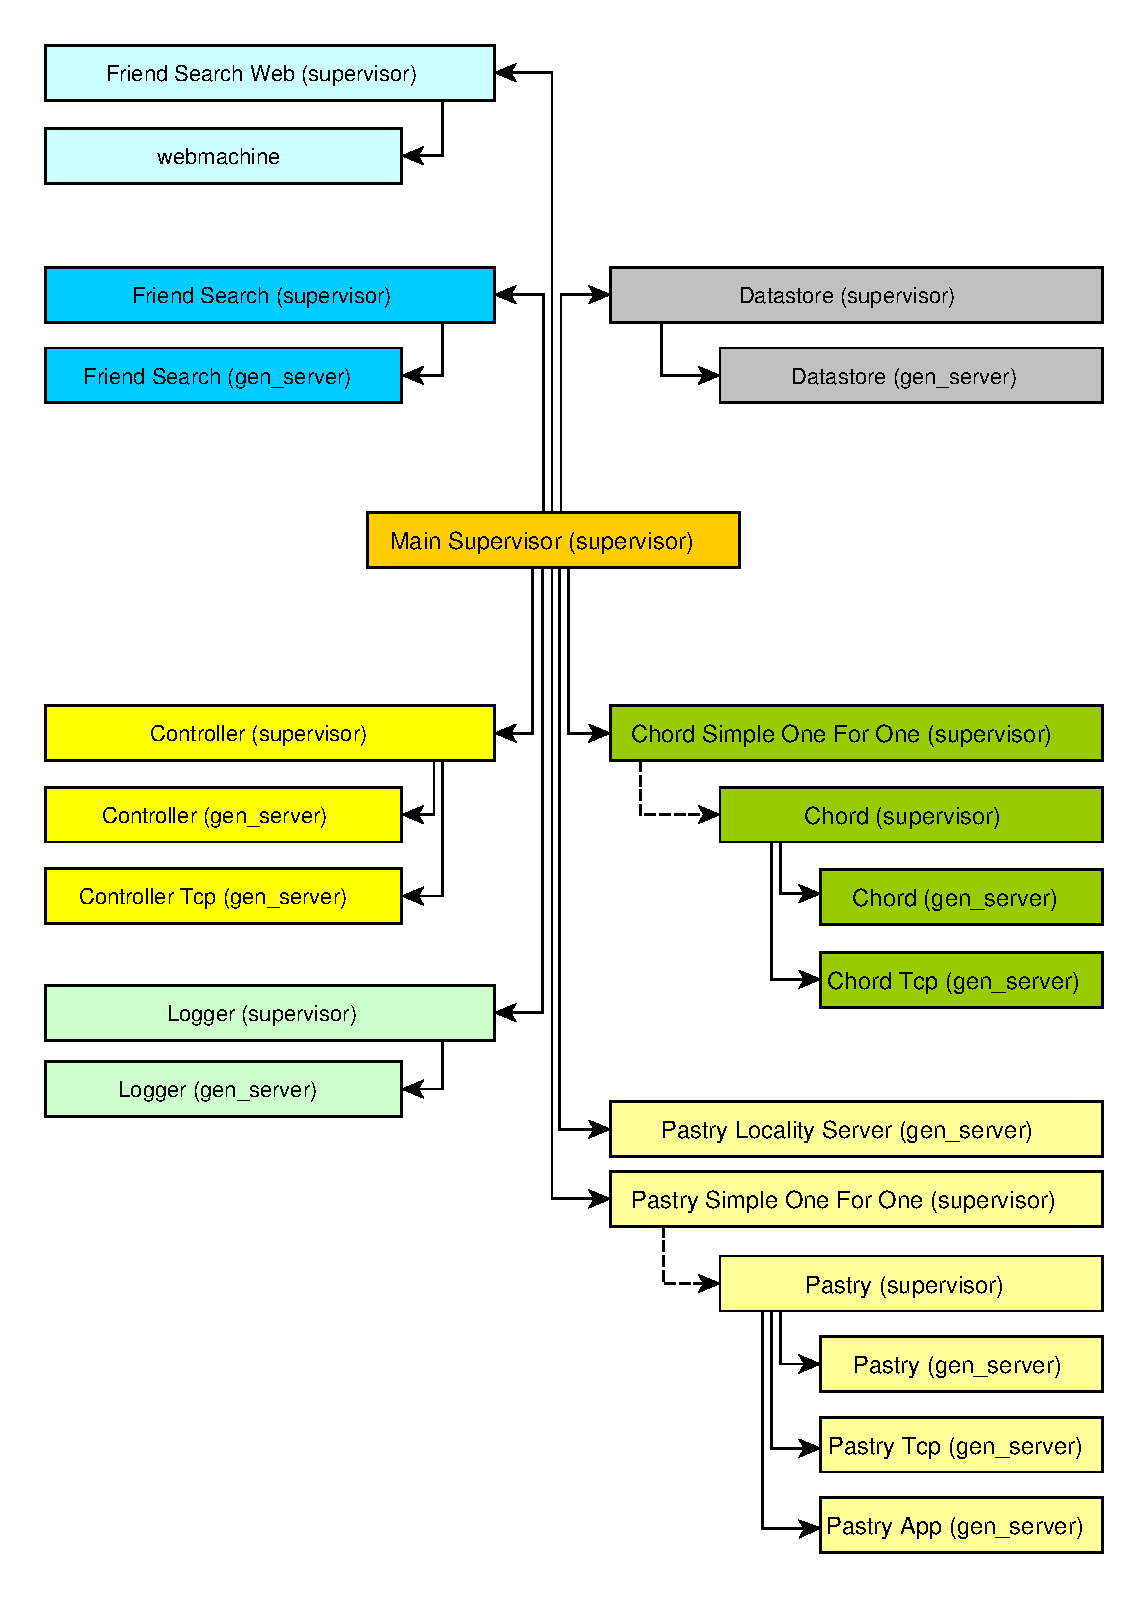
\includegraphics[width=0.9\linewidth]{illustrations/ClientSupervisionTree.eps}
\caption{Shows the full supervision tree of all the components}
\label{supervisionTree}
\end{center}
\end{figure}

%   How it all fits together
%     Supervision hierarchy

Summary
